\documentclass{beamer}
% AnnArbor  Antibes  Bergen  Berkeley  Berlin  Boadilla  CambridgeUS  Copenhagen  Darmstadt  Dresden  Frankfurt  Goettingen  Hannover  Ilmenau  JuanLesPins  Luebeck  Madrid  Malmoe  Marburg  Montpellier  PaloAlto  Pittsburgh  Rochester  Singapore  Szeged  Warsaw  boxes  default 
\mode<presentation>
{
  \usetheme{Antibes}
  \setbeamercovered{transparent}
}

\usepackage[english]{babel}
\usepackage{times}
\usepackage{graphicx}           
\usepackage{xeCJK}       
\usepackage{fontspec}
\setsansfont{SimSun}

\title[Assignment 4] 
{人机交互作业}

\subtitle
{图标设计}

\author[Author] 
{束裕 \and 吴继鹏 \and 王旻 \and 王建冬}

\institute[Universities of Somewhere and Elsewhere] 
{
  Software Institute\\
  Nanjing University
}

\date[AFP 2003]
{HCI Presentations, 2014}

\subject{Theoretical Computer Science}
\AtBeginSubsection[]
{
  \begin{frame}<beamer>{Outline}
    \tableofcontents[currentsection,currentsubsection]
  \end{frame}
}
\begin{document}

\begin{frame}
  \titlepage
\end{frame}

\begin{frame}{Outline}
  \tableofcontents
\end{frame}

\section{Abstract}
\begin{frame}{这篇报告包括:}
  \begin{itemize}
  \item 移动文本块、复制文本块、查看临时存储的文本、插入一个文本块的图标设计
  \item 4个图标独立的评价
  \item 4个图标作为一个图标组的总体评价
  \end{itemize}
\end{frame}  


\section{移动文本块}
\subsection{图标设计}
\begin{frame}
  \begin{figure}[H]
  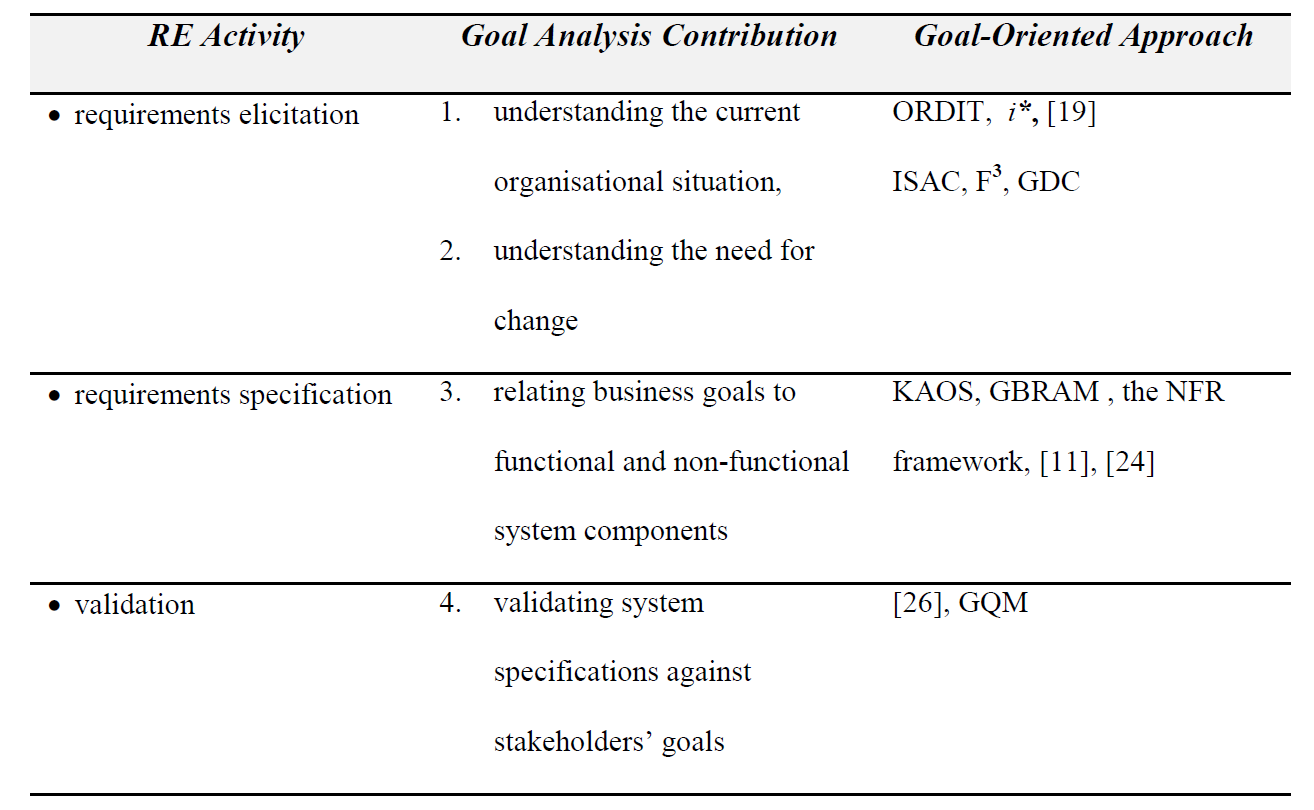
\includegraphics[width=1.4in]{img/1.PNG}
  \end{figure}
\end{frame}
\subsection{图标评价}
\begin{frame}
\begin{enumerate}
\item 图形清晰度:图标是一个$48\times 48$的图片。显示了一个文本经过一个箭头指向另一个文本的图片。
\item 释义的准确度: 图表显示了正确的概念。
\item 释义强度:图标率先表明了正确的概念,即文本移动。
\item 图形是否美观:还可以。
\end{enumerate}
\end{frame}


\section{插入文本块}
\begin{frame}
  \begin{figure}[H]
  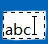
\includegraphics[width=1.4in]{img/2.jpg}
  \end{figure}
\end{frame}
\subsection{图标评价}
\begin{frame}
\begin{enumerate}
\item 复选框+abc表示可编辑的文本框
\item 鼠标‘I’图样表示插入
\item 图形简洁美观
\end{enumerate}
\end{frame}

\section{复制文本块}
\begin{frame}
  \begin{figure}[H]
  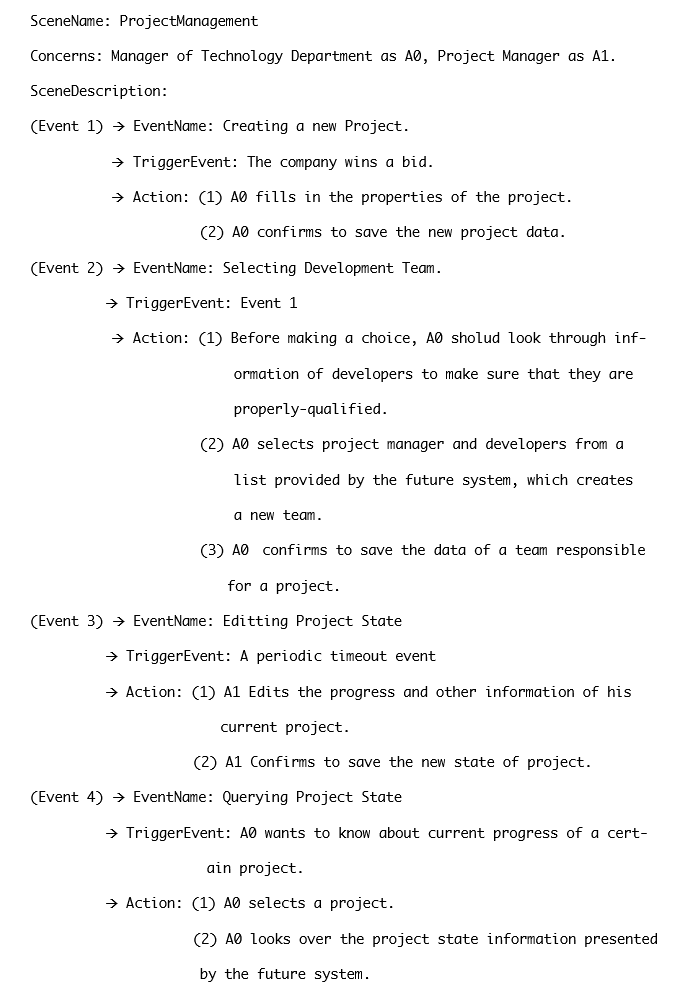
\includegraphics[width=1.4in]{img/3.bmp}
  \end{figure}
\end{frame}
\begin{frame}
\begin{enumerate}
\item 凸现复制的是文本,故用ABC象征文本
\item 用两个重叠的相同的文本块,让用户一眼看出是复制的意思
\item 图标释义准确,并与其他图标对比组有明显的区别
\item 图形简洁美观
\end{enumerate}
\end{frame}

\section{查看临时存储的文本}
\begin{frame}
  \begin{figure}[H]
  
\includegraphics[width=1.4in]{img/4.jpg}
  \end{figure}
\end{frame}
\begin{frame}
  \begin{enumerate}
  \item 用“软盘”作背景表示存储
  \item 用“眼镜”图案表示“查看”
  \item 用T表示文本
  \item 用代表事务的图像使得图标易识别
  \item 图标简洁美观
  \item 图标释义准确,与其他图标对比组有明显的区别
  \end{enumerate}
\end{frame}


\section{图标组评价}
\subsection{对比组的区别}
\begin{frame}
\begin{enumerate}
\item 4个图标都完全不同,作为一个图标组,相互之间是不会混淆的。\pause
\item 移动文本和复制是最有可能被设计得相似的,我们的设计中,前者是两个相距较远的文本,一个通过一个弯曲且逐渐变粗的箭头指向另一个,体现移动的动态感。而复制则是通过两个完全一样的文本,一个累加在另一个的上方,相互重叠,体现复制,符合传统上用户对“复制”这一概念的认知。
\end{enumerate}
\end{frame}
\subsection{对比组的关联}
\begin{frame}
\begin{enumerate}
\item 配色上统一采用蓝、白以及少量灰色,表明这一组按钮是同一个应用程序中的图标,且功能属于同一领域。\pause
\item 采用鲜艳色块作为图标,可以让狭小的空间$48\times48$发挥出最大的辨识度。\pause
\item 采用鲜艳色块作为图标,还可以明确地指明图标的边界。\pause
\item 采用扁平化设计,舍弃一切不必要的羽化,阴影,最大程度上突出图标的主题,简洁而有力。
\end{enumerate}
\end{frame}


\end{document}


